\chapter{Конструкторская часть}

В данном разделе приводится проектирование базы данных:
представлены её основные сущности и связи в виде ER-диаграммы,
определены ограничения целостности, описана ролевая модель,
а также приведена диаграмма классов для отражения структуры и взаимодействия элементов системы.

\section{Формализация сущностей системы}

На основе анализа предметной области, проведённого в предыдущем разделе, выделены ключевые сущности разрабатываемой базы данных. Каждая сущность представлена в виде таблицы, содержащей атрибуты с указанными типами данных, ограничениями целостности и связями с другими таблицами.

В реализуемой базе данных выделены следующие таблицы:

\begin{itemize}
    \item \textbf{Users} -- таблица пользователей системы;
    \item \textbf{Categories} -- таблица категорий датасетов;
    \item \textbf{Datasets} -- таблица с основной информацией о датасетах;
    \item \textbf{Dataset\_Versions} -- таблица версий датасетов;
    \item \textbf{Metadata} -- таблица метаданных, связанных с версиями датасетов;
    \item \textbf{Subscriptions} -- таблица подписок пользователей на датасеты;
    \item \textbf{Reviews} -- таблица отзывов и оценок пользователей;
    \item \textbf{Notifications} -- таблица уведомлений пользователей.
\end{itemize}

\clearpage
На рисунке~\ref{img:ernotchlen} представлена диаграмма сущность-связь базы данных

\begin{figure}[H]
	\centering
	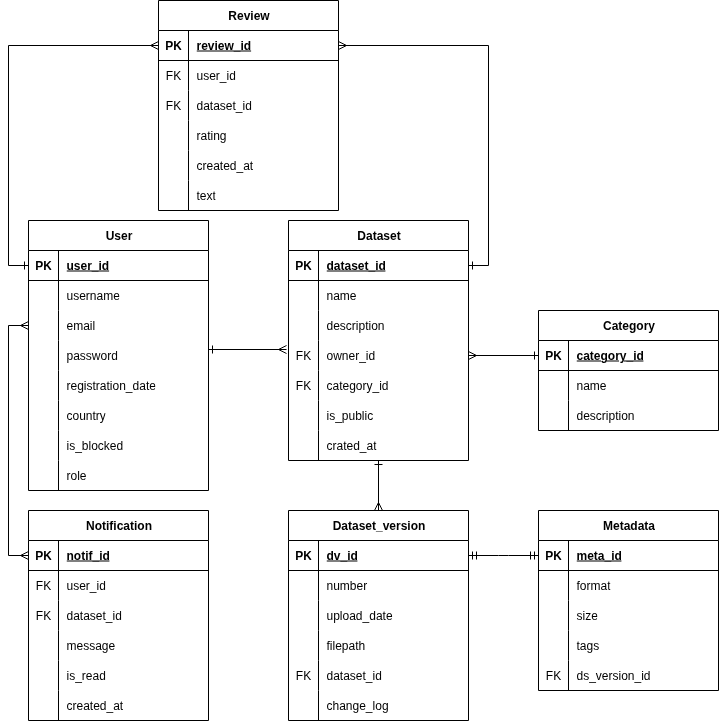
\includegraphics[scale=0.6]{images/er_not_chlen.drawio}
	\caption{ER-диаграмма базы данных}
	\label{img:ernotchlen}
\end{figure}

\clearpage
В таблицах~\ref{tab:users}~--~\ref{tab:notifications} приведены поля таблиц базы данных.

\subsubsection*{Таблица Users}

\begin{table}[H]
\centering
\caption{Атрибуты таблицы Users}
\label{tab:users}
\renewcommand{\arraystretch}{1.3}
\begin{tabular}{|p{3.5cm}|p{3cm}|p{4cm}|p{4.5cm}|}
\hline
\textbf{Атрибут} & \textbf{Тип} & \textbf{Ограничение} & \textbf{Описание} \\
\hline
id & целое число & первичный ключ & Уникальный идентификатор пользователя \\
\hline
username & строка & обязательное поле & Имя пользователя \\
\hline
email & строка & обязательное поле, уникальное значение & Электронная почта пользователя \\
\hline
password & строка & обязательное поле & Хеш пароля пользователя \\
\hline
registration\_date & дата/время & обязательное поле, значение по умолчанию: текущие дата и время & Дата и время регистрации \\
\hline
country & строка & обязательное поле & Страна пользователя \\
\hline
is\_blocked & логический & обязательное поле, значение по умолчанию: \texttt{false} & Статус блокировки пользователя \\
\hline
role & строка & обязательное поле, допустимые значения: \textit{guest}, \textit{user}, \textit{admin} & Роль пользователя в системе \\
\hline
\end{tabular}
\end{table}

\subsubsection*{Таблица Categories}

\begin{table}[H]
\centering
\caption{Атрибуты таблицы Categories}
\label{tab:categories}
\renewcommand{\arraystretch}{1.3}
\begin{tabular}{|p{3.5cm}|p{3cm}|p{4cm}|p{4.5cm}|}
\hline
\textbf{Атрибут} & \textbf{Тип} & \textbf{Ограничение} & \textbf{Описание} \\
\hline
id & целое число & первичный ключ & Уникальный идентификатор категории \\
\hline
name & строка & обязательное поле, уникальное значение & Название категории \\
\hline
description & текст & поле может отсутствовать & Описание категории \\
\hline
\end{tabular}
\end{table}

\subsubsection*{Таблица Datasets}

\begin{table}[H]
\centering
\caption{Атрибуты таблицы Datasets}
\label{tab:datasets}
\renewcommand{\arraystretch}{1.3}
\begin{tabular}{|p{3.5cm}|p{3cm}|p{4cm}|p{4.5cm}|}
\hline
\textbf{Атрибут} & \textbf{Тип} & \textbf{Ограничение} & \textbf{Описание} \\
\hline
id & целое число & первичный ключ & Уникальный идентификатор датасета \\
\hline
name & строка & обязательное поле & Название датасета \\
\hline
description & текст & поле может отсутствовать & Краткое описание датасета \\
\hline
owner\_id & целое число & внешний ключ & Владелец датасета \\
\hline
category\_id & целое число & внешний ключ & Категория датасета \\
\hline
is\_public & логический & обязательное поле, значение по умолчанию: \texttt{false} & Признак публичного доступа \\
\hline
created\_at & дата/время & обязательное поле, значение по умолчанию: текущие дата и время & Дата создания \\
\hline
\end{tabular}
\end{table}

\subsubsection*{Таблица Dataset\_Versions}

\begin{table}[H]
\centering
\caption{Атрибуты таблицы Dataset\_Versions}
\label{tab:dataset_versions}
\renewcommand{\arraystretch}{1.3}
\begin{tabular}{|p{3.5cm}|p{3cm}|p{4cm}|p{4.5cm}|}
\hline
\textbf{Атрибут} & \textbf{Тип} & \textbf{Ограничение} & \textbf{Описание} \\
\hline
id & целое число & первичный ключ & Уникальный идентификатор версии \\
\hline
number & строка & обязательное поле & Номер версии \\
\hline
upload\_date & дата/время & обязательное поле, значение по умолчанию: текущие дата и время & Дата загрузки версии \\
\hline
filepath & текст & обязательное поле & Путь к файлу версии \\
\hline
dataset\_id & целое число & внешний ключ & Датасет, к которому относится версия \\
\hline
change\_log & текст & поле может отсутствовать & Описание изменений в версии \\
\hline
\end{tabular}
\end{table}

\subsubsection*{Таблица Metadata}

\begin{table}[H]
\centering
\caption{Атрибуты таблицы Metadata}
\label{tab:metadata}
\renewcommand{\arraystretch}{1.3}
\begin{tabular}{|p{3.5cm}|p{3cm}|p{4cm}|p{4.5cm}|}
\hline
\textbf{Атрибут} & \textbf{Тип} & \textbf{Ограничение} & \textbf{Описание} \\
\hline
id & целое число & первичный ключ & Уникальный идентификатор метаданных \\
\hline
format & строка & обязательное поле & Формат данных (например, CSV, JSON и др.) \\
\hline
size & целое число & обязательное поле, значение должно быть положительным & Размер в байтах \\
\hline
tags & текст & поле может отсутствовать & Список ключевых слов (тегов) \\
\hline
\makecell[l]{dataset\\version\\id} & целое число & внешний ключ & Версия датасета, к которой относятся метаданные \\
\hline
\end{tabular}
\end{table}

\subsubsection*{Таблица Subscriptions}

\begin{table}[H]
\centering
\caption{Атрибуты таблицы Subscriptions}
\label{tab:subscriptions}
\renewcommand{\arraystretch}{1.3}
\begin{tabular}{|p{3.5cm}|p{3cm}|p{4cm}|p{4.5cm}|}
\hline
\textbf{Атрибут} & \textbf{Тип} & \textbf{Ограничение} & \textbf{Описание} \\
\hline
user\_id & целое число & внешний ключ, составной первичный ключ & Пользователь, оформивший подписку \\
\hline
dataset\_id & целое число & внешний ключ, составной первичный ключ & Датасет, на который оформлена подписка \\
\hline
created\_at & дата/время & обязательное поле, значение по умолчанию: текущие дата и время & Дата создания подписки \\
\hline
\end{tabular}
\end{table}

\subsubsection*{Таблица Reviews}

\begin{table}[H]
\centering
\caption{Атрибуты таблицы Reviews}
\label{tab:reviews}
\renewcommand{\arraystretch}{1.3}
\begin{tabular}{|p{3.5cm}|p{3cm}|p{4cm}|p{4.5cm}|}
\hline
\textbf{Атрибут} & \textbf{Тип} & \textbf{Ограничение} & \textbf{Описание} \\
\hline
id & целое число & первичный ключ & Уникальный идентификатор отзыва \\
\hline
user\_id & целое число & внешний ключ & Пользователь, оставивший отзыв \\
\hline
dataset\_id & целое число & внешний ключ & Датасет, к которому относится отзыв \\
\hline
rating & целое число & обязательное поле, допустимый диапазон: от 1 до 5 & Оценка качества датасета \\
\hline
created\_at & дата/время & обязательное поле, значение по умолчанию: текущие дата и время & Дата создания отзыва \\
\hline
text & текст & поле может отсутствовать & Текстовый комментарий \\
\hline
\end{tabular}
\end{table}

\subsubsection*{Таблица Notifications}

\begin{table}[H]
\centering
\caption{Атрибуты таблицы Notifications}
\label{tab:notifications}
\renewcommand{\arraystretch}{1.3}
\begin{tabular}{|p{3.5cm}|p{3cm}|p{4cm}|p{4.5cm}|}
\hline
\textbf{Атрибут} & \textbf{Тип} & \textbf{Ограничение} & \textbf{Описание} \\
\hline
id & целое число & первичный ключ & Уникальный идентификатор уведомления \\
\hline
user\_id & целое число & внешний ключ & Пользователь, которому адресовано уведомление \\
\hline
dataset\_id & целое число & внешний ключ & Датасет, связанный с уведомлением \\
\hline
message & текст & обязательное поле & Текст уведомления \\
\hline
is\_read & логический & обязательное поле, значение по умолчанию: \texttt{false} & Признак прочтения уведомления \\
\hline
created\_at & дата/время & обязательное поле, значение по умолчанию: текущие дата и время & Дата создания уведомления \\
\hline
\end{tabular}
\end{table}

\section{Функция вычисления среднего рейтинга датасета}

В рамках базы данных реализована функция вычисления среднего значения
рейтингов для конкретного датасета.
На вход функция принимает идентификатор
датасета. Если оценки присутствуют, функция
вычисляет их среднее арифметическое в диапазоне от 1 до 5. В случае отсутствия
оценок результатом работы функции
является \texttt{0.0}.

\clearpage
На рисунке~\ref{fig:avg_rating_func} представлено описание алгоритма функции
вычисления среднего рейтинга датасета.

\begin{figure}[H]
    \centering
    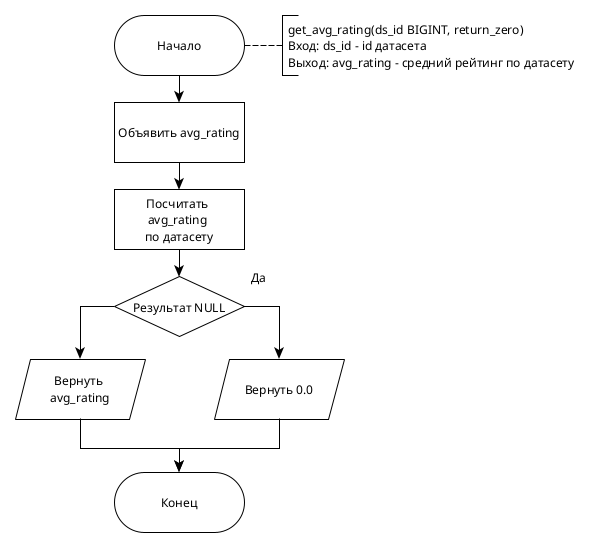
\includegraphics[width=0.9\textwidth]{images/avg}
    \caption{Схема алгоритма функции вычисления среднего рейтинга}
    \label{fig:avg_rating_func}
\end{figure}

\section{Описание триггера базы данных}

В базе данных реализован триггер, который срабатывает после добавления новой записи
в таблицу \texttt{datasets}. Его назначение --- автоматизация служебных действий
при создании датасета: проверка владельца, настройка видимости, создание подписки,
инициализация версии и уведомление владельца.

\clearpage
На рисунке~\ref{fig:trg_after_insert_datasets} представлено описание алгоритма триггера.

\begin{figure}[H]
    \centering
    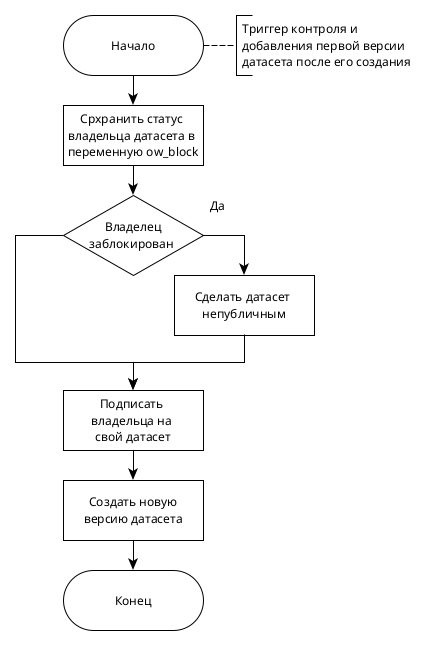
\includegraphics[scale=0.6]{images/trig}
    \caption{Схема алгоритма работы триггера базы данных}
    \label{fig:trg_after_insert_datasets}
\end{figure}

\section{Ролевая модель}

Для обеспечения безопасности и управления доступом к данным в системе
разработана ролевая модель. Она определяет права доступа для различных
категорий пользователей, что позволяет ограничить доступ к данным в зависимости
от их роли, минимизировать риски несанкционированного изменения информации и
упростить администрирование системы.

\subsubsection{Роль Guest (Гость)}

Гость --- это неавторизованный пользователь, который может только
просматривать общедоступную информацию. Права:
\begin{itemize}
  \item SELECT --- над таблицей \texttt{datasets} (просмотр только записей с атрибутом \texttt{is\_public = TRUE});
  \item SELECT --- над таблицей \texttt{categories} (просмотр категорий).
\end{itemize}

Гость не имеет доступа к данным о пользователях, подписках, отзывах,
уведомлениях и версиях датасетов. Это обеспечивает защиту персональных данных и
ограничивает функционал незарегистрированных пользователей.

\subsubsection{Роль User (Зарегистрированный пользователь)}

Зарегистрированный пользователь имеет более широкий набор прав: он может
подписываться на датасеты, оставлять отзывы и управлять собственными наборами
данных. Права:
\begin{itemize}
  \item SELECT --- над таблицами \texttt{datasets}, \texttt{categories}, \texttt{dataset\_versions}, \texttt{metadata} (просмотр информации о датасетах);
  \item SELECT, INSERT --- над таблицей \texttt{subscriptions} (оформление подписки и просмотр своих подписок);
  \item SELECT, INSERT --- над таблицей \texttt{reviews} (просмотр и добавление отзывов);
  \item SELECT, INSERT --- над таблицей \texttt{notifications} (получение и отметка уведомлений);
  \item SELECT, INSERT, UPDATE, DELETE --- над таблицей \texttt{datasets}, но только для записей, где он является владельцем (\texttt{owner\_id = current\_user});
  \item SELECT, INSERT, UPDATE, DELETE --- над таблицей \texttt{dataset\_versions} для версий собственных датасетов;
  \item SELECT, INSERT, UPDATE, DELETE --- над таблицей \texttt{metadata}, связанной с собственными версиями датасетов.
\end{itemize}

Таким образом, пользователь имеет полный контроль только над своими данными, а
над чужими датасетами и их версиями --- только права чтения, если они публичны.

\subsubsection{Роль Admin (Администратор)}

Администратор --- это пользователь с полным доступом ко всем объектам системы.
Права:
\begin{itemize}
  \item SELECT, INSERT, UPDATE, DELETE --- над таблицей \texttt{users} (управление учётными записями);
  \item SELECT, INSERT, UPDATE, DELETE --- над таблицами \texttt{datasets}, \texttt{dataset\_versions}, \texttt{metadata} (полный контроль над хранимыми наборами данных);
  \item SELECT, INSERT, UPDATE, DELETE --- над таблицами \texttt{categories}, \texttt{subscriptions}, \texttt{reviews}, \texttt{notifications};
  \item Возможность блокировки пользователей (\texttt{is\_blocked = TRUE});
  \item Возможность изменения ролей пользователей (\texttt{role} в таблице \texttt{users}).
\end{itemize}

Администратор отвечает за модерацию содержимого, управление пользователями,
категориями и обеспечение корректного функционирования системы в целом.
\section*{Вывод}

В конструкторской части была спроектирована структура базы данных:
выделены ключевые сущности и их атрибуты, определены ограничения целостности
и взаимосвязи между таблицами. Построена ER-диаграмма, наглядно отражающая
архитектуру системы. Для обеспечения безопасности и разграничения прав доступа
разработана ролевая модель, включающая роли гостя, зарегистрированного
пользователя и администратора. Описанные элементы создают основу для дальнейшей
реализации и тестирования базы данных и прикладного программного обеспечения.